
\documentclass{article}

\usepackage{graphicx}
\usepackage[centerlast,small,sc]{caption}
\usepackage{alltt}
\usepackage{url}
\usepackage{tabularx}
\usepackage{hyperref}
\usepackage{listings}
\usepackage{longtable}
\usepackage[utf8]{inputenc}
\usepackage[italian]{babel}

%\newenvironment{prettytablex}[1]{\vspace{0.3cm}\noindent\tabularx{\linewidth}{@{\hspace{\parindent}}#1@{}}}{\endtabularx\vspace{0.3cm}}
%\newenvironment{prettytable}{\prettytablex{l X}}{\endprettytablex}

\lstset{ %
  language=Java,                % the language of the code
  basicstyle=\footnotesize, 
  breaklines=true                % sets automatic line breaking
}

\title{\huge\sffamily\bfseries Descrizione del sistema e Analisi del Rischio}
\author{Nicolò Marchi \and Alessandro Gottoli \and Mattia Peretti}
\date{\today}


\begin{document}
\maketitle

\tableofcontents
\listoffigures
\pagebreak


\section{Descrizione del Sistema}

\subsection{Panoramica del sistema}

L'assegnamento per il laboratorio di Sicurezza delle Reti consisteva nell'implementazione di una Certificate Authority (in seguito, CA) riguardante una fittizia compagnia di nome \emph{iMovies}, che vuole offrire ai suoi clienti dei servizi basati su PKI (Public Key Infrastructure).
Le direttive per l'implementazione di tale CA sono descritte dal libro di testo \cite{applied security} adottato.

Una PKI è una infrastruttura che permette di riconoscere a chi appartengono determinate chiavi pubbliche. In questa infrastruttura vi sarà una Certificate Authority, che firmando certificati certifica che la chiave pubblica $pk$ appartiene alla persona $P$.
Per firmare questo certificato la CA si occuperà di verificare che la persona che ha richiesto certificazione sia realmente chi dice di essere, dopodichè ne firmerà il certificato.
La persona $P$ quindi ora può distribuire la propria chiave pubblica certificata.

La nostra implementazione di iMovies permette agli utenti (già inseriti nel database fornito) la creazione e la firma di certificati che verranno poi usati per la comunicazione sicura tramite e-mail.
Questi certificati avranno una durata di 6 mesi, con la data di inizio e fine validità che deve essere scelta dall'utente in fase di creazione. Questa scelta è dovuta al fatto che non ci sembrava una scelta ottimale lasciare che si potessero creare o solo un certificato con lo stesso Subject\footnote{Il campo Subject identifica l'entità associata alla chiave pubblica memorizzata nel campo Public Key del Subject. Il nome del Subject può essere trasportato nel campo Subject.}, o $n$ certificati con Subject uguale e date di validità standard (cioè dal giorno di creazione fino a 365 giorni dopo).

L'architettura del sistema è composta da due parti:
\begin{itemize}
\item una macchina virtuale di nome \textbf{ServerIMovies}.
\item una macchina virtuale di nome \textbf{ClientIMovies}.
\end{itemize}

La web application è stata scritta utilizzando il framework Java Server Faces (JSF) per permettere una maggiore attenzione al backend Java attraverso una più facile implementazione del frontend grafico composto da pagine xhtml (create utilizzando le librerie di componenti grafici \emph{Primefaces}\footnote{Per maggiori informazioni, \url{http://www.primefaces.org}}.).

Per la gestione del database ci si è affidati al  Relational Database Management System MySql.
Per quanto riguarda la creazione, la firma, la revoca, e tutte le operazioni di gestione dei certificati ci si è affidati al toolkit \emph{OpenSSL}\footnote{Implementazione open-source dei protocolli SSL/TLS. \url{http://www.openssl.org/}}. 

Infine, per gli archivi di backup dei dati è stato usato il semplice tool \emph{tar}, presente in ogni distribuzione Unix. Per lo scheduling dei backup è stato usato il tool \emph{cron}, e per il download remoto dei backups ci siamo affidati a \emph{FileZilla} 

%This description should provide a high-level
%overview of the system, e.g., suitable for managers, that complements
%the more technical description that follows.


\subsection{Funzionalità del Sistema}
\subsubsection*{Login}
\begin{figure}[h!]
\centering
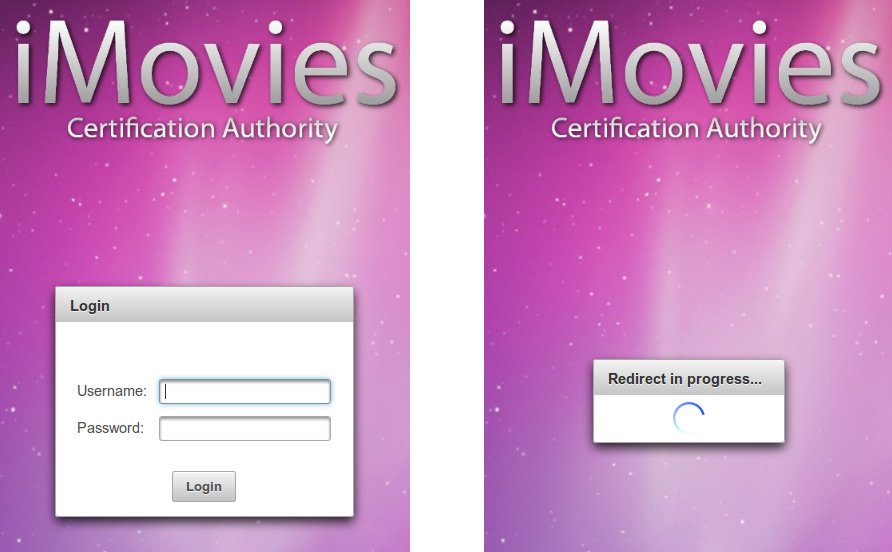
\includegraphics[width=\textwidth]{img/login}
\caption{Differenza tra il login che viene mostrato al cliente (immagine a sinistra) e il login automatico tramite certificato per l'amministratore.}
\end{figure}
Il sistema offre principalmente due possibilità di login. Una possibilità consiste nel connettersi al portale attraverso un certificato PKCS\#12 riconosciuto dalla CA iMovies, che permette di bypassare il controllo delle credenziali nel database (dato che si presume che il certificato sia in mano al proprietario dello stesso).
\par La seconda modalità consiste in un canonico form di login nel quale l'utente è chiamato ad inserire lo username e la password. Per quest'ultimo campo, verrà calcolato il corrispondente hash SHA-1 e tale valore sarà utilizzato nel confronto con gli hash delle password salvati nel database.
\subsubsection*{Modifica informazioni personali}
\begin{figure}[h!]
\centering
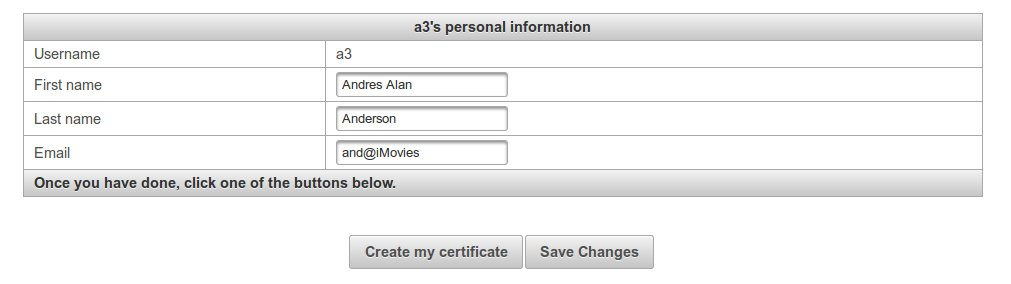
\includegraphics[width=\textwidth]{img/edit}
\caption{Le tabella contenente le informazioni personali modificabili dell'utente \emph{a3}.}
\end{figure}
Il portale offre agli utenti la possibilità di modificare le informazioni personali precedentemente salvate nel database. Si possono modificare tutti i campi, ad eccezione del campo username, che è fisso e ha il ruolo di primary key nella tabella relativa agli utenti nel database.
\subsubsection*{Rilascio di certificati}
Ad ogni utente viene fornita la possibilità di creare certificati. Alla creazione di un certificato viene generata una chiave privata con crittografia a 4096 bit e crittata con DES3 e una password inserita dall'utente. Dopodiché viene generato e firmato il certificato relativo, con i dati dell'utente salvati nel database.
\subsubsection*{Revoca dei certificati}
Nella sezione di management dei certificati viene fornita la possibilità di revocare selettivamente i certificati dell'utente. Quando un certificato viene revocato, viene generata nuovamente la Certificate Revocation List della Certificate Authority.
\subsubsection*{Download dei certificati}
Viene fornita la possibilità di scaricare i certificati e le relative chiavi private in formato PKCS\#12. Quando si richiede il download del certificato il sistema richiederà all'utente la password usata durante la creazione della chiave privata, e una nuova password che sarà usata per l'esportazione del certificato PKCS\#12. QUest'ultima password dovrà essere inserita quando si importerà il certificato all'interno di un browser.
\subsubsection*{Eliminazione dei certificati}
\begin{figure}[h!]
\centering
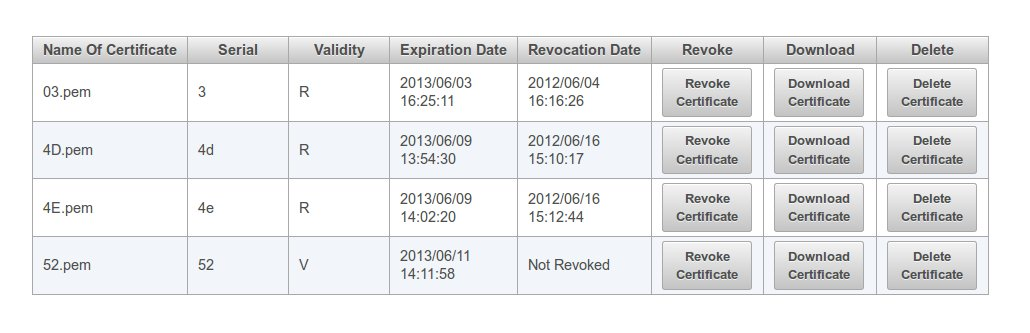
\includegraphics[width=\textwidth]{img/revokedownload}
\caption{Tabella per il download, la revoca e l'eliminazione dei certificati.}
\end{figure}
Quando un utente sceglie di rimuovere un certificato, innanzi tutto quest'ultimo verrà revocato; dopodiché verrà eliminata la chiave privata associata al certificato, e il certificato stesso.
\subsubsection*{Amministrazione del portale}
\begin{figure}[h!]
\centering
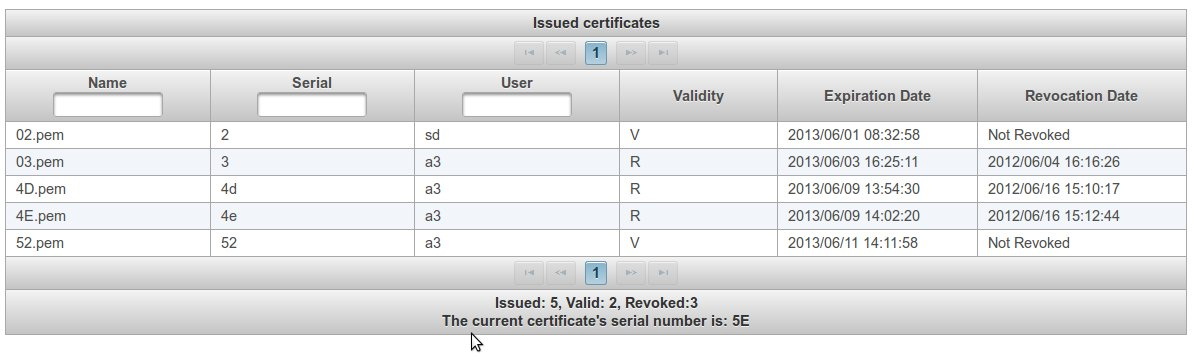
\includegraphics[width=\textwidth]{img/certs}
\caption{Tabella per la visualizzazione di tutti i certificati rilasciati con contatori e prossimo serial number.}
\end{figure}
L'amministratore del portale accede al frontend di amministrazione solamente con un certificato PKCS\#12 già in suo possesso. Attraverso le pagine dell'area amministrativa,  l'amministratore può vedere quanti e quali certificati sono stati rilasciati, quanti e quali certificati sono stati revocati, e il valore corrente del serial number\footnote{il valore del numero esadecimale che verrà assegnato al prossimo certificato generato}.
\par Inoltre viene effettuato un log di tutti gli accessi al sito, compresi gli accessi effettuati passando attraverso le backdoor.
\subsubsection*{Backup dei dati}
Il sistema esegue un periodico backup di tutte le chiavi private e di tutti i certificati. I backup sono in realtà due, uno totale che viene eseguito ogni settimana il venerdì alle ore 11.00, mentre un backup incrementale che viene eseguito tutte le ore al minuto 40. In entrambi i casi viene generato un archivio con il comando Unix ``tar''.
\par Vi è poi un server ftp che permette ad un amministratore di scaricare da remoto i backups. L'accesso da ftp è limitato solamente alla cartella ove vi sono i backups.

\subsection{Componenti e Sottosistemi}
\subsubsection*{Java Server Faces}
Come già accennato, per l'implementazione del portale è stata usata la tecnologia di Java Server Faces. JSF, acronimo di Java Server Faces può essere considerata un framework per lo sviluppo di web application basate su Java. \'E basato sul design pattern architetturale Model-View-Controller (MVC) ed è descritto da un documento di specifiche (JSR 127) alla cui stesura hanno partecipato aziende quali IBM, Oracle Corporation, Siemens e Sun Microsystems. Il suo scopo è di semplificare lo sviluppo dell'interfaccia utente (UI) di una applicazione Web.
\par A grandi linee il funzionamento del framework JSF si basa su un file di configurazione XML ({\tt faces-config.xml}) in cui vengono definite le viste (sostanzialmente pagine JSP che sfruttano la \emph{taglibrary faces}) e i controllori. Le singole implementazioni sfruttano una servlet di base {\tt FacesServlet} o un filtro il cui mapping è normalmente {\tt /faces/*} o {\tt *.faces}. La {\tt FacesServlet} deve essere registrata nel file XML ({\tt web.xml}) della web application.
\subsubsection*{PrimeFaces}
\begin{figure}[h!]
\centering

\includegraphics[width=.5\textwidth]{img/prime}
\caption{Il logo delle librerie Primefaces.}
\end{figure}
Le librerie Primefaces costituiscono una serie di componenti grafici utilizzabili all'interno di una web application Jsf.
PrimeFaces è una suite open source utilizzabile con il framework Java Server Faces, esplicitamente pensata per realizzare i componenti presentazionali di una applicazione web enterprise: editor HTML, finestre di dialogo, meccanismi per l'auto-completamento, grafici e calendari, drag \& drop, integrazione di mappe google e molto altro.
\par La suite offre supporto sia ad ajax che al rendering parziale delle pagine web, grazie ad una integrazione nativa con {\tt jquery}. L'aspetto grafico dei componenti si basa su {\tt JQuery UI}: è quindi possibile personalizzarlo attraverso lo skin framework \emph{Theme Roller}, o utilizzare un discreto insieme di temi predefiniti. Da segnalare infine la presenza di uno \emph{User Interface Kit} per la realizzazione di applicazioni Web orientate ai dispositivi mobili (iPhone, Android, etc.), di semplice e veloce configurazione.
%Per tale motivo, in unione con gli ottimi componenti grafici forniti dalle librerie Primefaces, la nostra scelta è ricaduta su questo tipo di tecnologia.

\subsubsection*{Macchine Virtuali}
Come già accennato, le macchine virtuali create sono due,  installate tramite il software open source \emph{VirtualBox}, e sono suddivise in macchina server e macchina client.
\par La macchina client si chiama \textbf{ClientIMovies}, e consiste in un'installazione della distribuzione Linux \emph{Ubuntu 12.04 LTS} per architetture \emph{amd64}. Le specifiche tecniche della macchina consistono in un hard disk dinamico della dimensione massima di 8 Gigabyte, 1024 MB di RAM e 12 MB di memoria dedicata alla parte grafica. La macchina ha la possibilità di vedere dispositivi USB e di condividere cartelle. Vi è una sola scheda di rete impostata in modo da essere connessa in una rete interna chiamata \emph{INFSEC}. Nella macchina sono presenti due utenti principali:
\begin{enumerate}
\item utente \emph{admin}: amministratore del portale iMovies. Nell'utenza è già installato il certificato PKCS\#12 relativo all'amministratore che permette il login rapido alla sezione di amministrazione del portale, un client ftp (più precisamente FileZilla) per il download dei backups da remoto, e un demone SSH per la connessione remota. 
\item utente \emph{client}: rappresenta un cliente del portale iMovies. L'utenza non ha caratteristiche particolari.
\end{enumerate} 
\par La macchina server si chiama \textbf{ServerIMovies}, e consiste in un'installazione della distribuzione Linux \emph{Ubuntu Server 12.04 LTS} sempre per architetture \emph{amd64}. Le specifiche tecniche della macchina consistono in un hard disk dinamico della dimensione massima di 8 Gigabyte, 512 MB di RAM e 12 MB di memoria dedicata alla parte grafica. La macchina ha la possibilità di vedere solamente cartelle condivise. Vi è una sola scheda di rete impostata in modo da essere connessa in una rete interna chiamata \emph{INFSEC}.
Al suo interno troviamo installati tutti i servizi utili al mantenimento e all'esecuzione del portale.
\par Le macchine virtuali si trovano connesse tra loro in una rete interna, con assegnati come indirizzi IP 192.168.1.11 per la macchina server, mentre 192.168.1.10 per la macchina client.
\subsubsection*{Web Server}
Per poter utilizzare le Java Server Faces, abbiamo dovuto scegliere (in maniera quasi obbligata) il web server \emph{Apache Tomcat 7.0}, ultima versione del noto web container.
Tomcat è un contenitore servlet open source sviluppato dalla Apache Software Foundation. Implementa le specifiche Java Server Pages (JSP) e Servlet, fornendo quindi una piattaforma per l'esecuzione di applicazioni Web sviluppate nel linguaggio Java. La sua distribuzione standard include anche le funzionalità di web server tradizionale, che corrispondono al prodotto Apache.
\subsubsection*{vsftpd}
\subsubsection*{test}

 --------------------not finished
List all system components, subdivided, for example, into
  categories such as platforms, applications, data records, etc. For
  each component, state its relevant properties.


\subsection{Interfacce}
\subsubsection*{login.xhtml}
La pagina di login si presenta molto semplice, con un semplice form di login dove inserire username e password. Dalla pagina di login si passa sempre e comunque, anche se si ha un certificato PKCS\#12 riconosciuto. In quest'ultimo caso nella pagina viene effettuato il controllo del certificato e il redirect alla pagina di amministrazione (in caso di certificato dell'admin) o nella pagina dell'user, con i dati dell'utente.
\subsubsection*{user.xhtml}
La pagina consiste in una semplice pagina di benvenuto dove vi è presente un menù di navigazione e un semplice messaggio di benvenuto. Da questa pagina l'utente può muoversi tra tutte le funzionalità del portale.
\subsubsection*{edit.xhtml}
\'E la pagina contenente tutte le informazioni dell'utente loggato nel sistema. Da questa pagina è possibile modificare le proprie informazioni personali (ad eccezione dello username), e sulla base di queste informazioni personali generare un certificato, selezionandone la data di inizio e fine, e inserendo una password per la chiave privata.
\subsubsection*{manageCertificates.xhtml}
Questa è la pagina adibita alla gestione dei certificati dell'utente. In questa pagina l'utente può vedere i suoi certificati, anche quelli revocati. Da qui può decidere se cancellare i certificati, revocarli o avviare la procedura di download, che genera il certificato PKCS\#12 a partire dalla chiave privata e dal certificato preso in esame.
\subsubsection*{admin.xhtml}
Questa è la sezione dedicata all'amministratore del portale. Da qui l'amministratore può muoversi attraverso un menù, per le varie sezioni dell'area amministrativa.
\subsubsection*{issued.xhtml}
L'amministratore in questa pagina può vedere tutti i certificati creati dagli utenti della CA. Può inoltre visualizzare il numero totale di certificati revocati, e il numero seriale corrente. Da un menù può inoltre muoversi nell'altra sezione dell'amministrazione, che è quella riguardante il controllo degli accessi.
\subsubsection*{aclog.xhtml}
Da questa pagina l'amministratore può vedere in tempo reale gli accessi al sito. Può vedere chi si è connesso, a che ora, e anche chi si è connesso passando attraverso le backdoor. La pagina offre inoltre la possibilità di esportare tutti i dati in formato \emph{.pdf} o \emph{.xls}.
\\ \\
---------------------------------------
possibile use case
------------------------
\\
\\

\subsection{Backdoors}

\subsubsection{Backdoor triviale}
Questa backdoor consiste nell'avere Apache Tomcat in ascolto su una porta particolare, scelta da noi, e cioè la porta 43567.
La porta è rilevabile tramite l'applicazione {\tt nmap} (Network Mapper). Cercando quindi di connettersi alla porta 43567 viene eseguito immediatamente il redirect verso il back-end di amministrazione del portale, dove verrà visualizzata una web shell (\emph{MindTerm}) in un pop-up, connessa in SSH alla macchina server con privilegi di root.
\\ \\
immagine sca nmap (sempre se lo facciamo funzionare)

\subsubsection{Backdoor complessa}
Questa backdoor consiste nell'implementazione di una semplice password segreta. Citando un film del 1983, ``Wargames'' diretto da John Badham, la backdoor consiste nell'inserire la parola "Joshua" nel solo campo password del form di login. La password inserita viene poi trasformata in un hash SHA-1.

All'interno del codice Java, nella classe relativa al controllo delle credenziali passate come input, vi è un campo privato, statico, e costante di nome \emph{magic}. Questo campo contiene l'hash SHA-1 della parola ``Joshua''. Quando nel form di login viene inserita la password e lo username resta vuoto, viene confrontato lo SHA-1 della parola inserita col campo \emph{magic}. Se il controllo da esito positivo viene fatto il redirect su una pagina contenente un'applet Java che avvia una shell, che connettendosi in SSH con le credenziali di Root, da accesso da super user sulla macchina server.

Riportiamo qui sotto lo spezzone di codice:

\begin{lstlisting}

(...)

private static final String magic="a9a2e8456bf9d58e91fe91cbfe10cad5211216c2";

(...)

if(SHAsum(password.getBytes()).equals(magic)){
	this.admin=true;
	log.aclog("backdoor user", 0);
	adminAccess();
	return;
}

(...)

\end{lstlisting}

\subsection{Materiale Aggiuntivo}

You may have additional sections according to your needs.


\section{Analisi del Rischio e Misure di Sicurezza}

\subsection{Information Assets}

Describe the relevant assets and their required security
  properties. For example, data objects, access restrictions,
  configurations, etc.

\subsection{Fonti delle minacce}

Le fonti delle minacce sono ciò che può minacciare la sicurezza della CA. Una fonte di minaccia potrebbe essere ad esempio un agente, che vuole qualcosa dalla CA, come ad esempio un certificato. Individuare gli agenti di minaccia è molto importante per poi poter individuare le fonti di minaccia.

Le fonti di minaccia principali per la CA, e anche per la maggior parte dei portali esistenti, si possono suddividere in alcune categorie:
\begin{itemize}
\item fonti che non hanno obiettivo specifico: le fonti di minaccia che non hanno un obiettivo specifico possono essere i virtus, gli worms, i trojans e le bombe logiche;
\item fonti interne: dipendenti, membri dello staff, personale, o chiunque abbia un qualche risentimento verso l'obiettivo;
\item fonti criminali: possono essere criminali solitari o associazioni di crimine organizzato, e avranno come obiettivo informazioni di valore per loro e per i loro traffici, come account bancari, carte di credito, o tutto ciò che si può convertire o sfruttare per guadagnare denaro;
\item fonte da aziende rivali: aziende che sono impegnate nella guerra delle informazioni o competitive intelligence. I partner e concorrenti rientrano in questa categoria;
\item fonte umana non intenzionale: incidenti, negligenza, disattenzione;
\item fonte umana intenzionale: Insider, outsider;
\item fonte naturale: catastrofi naturali di ogni tipologia, come terremoti, incendi, alluvioni, ecc.
\end{itemize}

Tenendo conto di tutte queste possibili fonti di minaccia, abbiamo stilato una lista di possibili agenti che possono attaccare o rappresentare fonte di minaccia per la nostra CA. Sono stati elencati in ordine dal più probabile al meno probabile, e sono:

\begin{enumerate}
\item L'attaccante motivato: rappresenta il pericolo maggiore; è un attaccante senza scrupoli che vuole a tutti i costi qualcosa dalla Certificate Authority, un qualcosa che non può avere in via ``legale''. Potrebbe essere un ex-dipendente arrabbiato, o un hacker pagato appositamente da qualcuno, o da qualche organizzazione criminale, per penetrare il sistema.
\item Malware automatico: programma o script, che è alla ricerca di vulnerabilità note, che poi riportano segnalazioni ad un sito di raccolta centrale.
\item Crackers: utenti che cercano di compromettere o eseguire deface ad applicazioni per un guadagno, per la notorietà o per un idea politica.
\item Hackers veri e propri: un ricercatore di sicurezza o un utente ordinario, che nota qualcosa di sbagliato con l'applicazione, e decide di proseguire nella scoperta della vulnerabilità, per poi creare immediatamente una patch e comunicare agli amministratori la falla trovata e la possibile soluzione.
\item Lo scopritore casuale: un utente normale che si imbatte in un errore funzionale nell'applicazione, semplicemente utilizzando un browser web, e guadagna l'accesso a informazioni privilegiate o funzionalità di livello superiore.
\end{enumerate}

Definite minacce e agenti, possiamo effettuare un'analisi dei rischi della nostra applicazione, basandoci sulle minacce che possono verificarsi contro la nostra Certificate Authority.

\subsection{Rischi e Contromisure}
In questa sezione cerchiamo di individuare i rischi principali di attacchi possibili alla CA iMovies.
Innanzi tutto già in fase di progettazione avevamo preso in considerazione possibili rischi e vulnerabilità di sistema, in modo da cercare di progettare un sistema sicuro già in partenza.
Infatti la scelta di utilizzare Java Server Faces è venuta anche da questa valutazione iniziale.

Dopodichè a lavoro ultimato si è deciso di cercare di migliorare ancora di più la sicurezza del sito, testandolo con alcuni tool automatici e con utenti scelti tra amici (come ad esempio Federico De Meo e Alberto Lovato). Oltre ad aiutarci nel testing della Certificate Authority ci hanno anche aiutato a svolgere alcuni attacchi presi dal Common Attack Pattern Enumeration and Classification (CAPEC)\footnote{\url{http://capec.mitre.org/}}.

Presentiamo ora i tool principali che abbiamo utilizzato per cercare eventuali falle nel sistema. Dopodichè nella parte successiva nelle tabelle presenti evidenzieremo come noi abbiamo considerato e valutato i livelli di rischio, probabilità e impatto delle vulnerabilità trovate e per cui abbiamo poi trovato una contromisura.

\subsubsection{Tools}
Una volta effettuata l'implementazione del sistema, sono stati utilizzati differenti tool per il test delle vulnerabilità del sistema.

\begin{itemize}
\item \textbf{Websecurify}\footnote{\url{http://www.websecurify.com}}\\
Websecurify è una potente applicazione per rilevare velocemente e in modo accurato le vulnerabilità di una web application.

L'applicazione è disponibile come plugin per browser e software standalone per sistemi Windows, Mac e Linux.

Data la release prematura disponibile per sistemi Linux è stato deciso di utilizzare il plugin per Google Chrome.

risultati...!

\item \textbf{Wapiti}\footnote{\url{http://www.ict-romulus.eu/web/wapiti/home}}\\
Wapiti è uno scanner di vulnerabilità di una web application.
Non esamina il codice sorgente delle pagine della web application ma si occupa di scansionare le pagine alla ricerca di form o campi di testo attraverso i quali eseguire delle injections. Per questo motivo, è definito come un \emph{fuzzer}\footnote{Un fuzzer è un software che sfrutta il fuzzing. Quest'ultimo è una tecnica di testing, automatica o semiautomatica, attraverso la quale vengono inviati input invalidi, inaspettati o casuali ad un programma con lo scopo di trovare vulnerabilità attraverso un monitoring delle risposte dello stesso.}.

La release di Wapiti utilizzata per questo test è la 2.2.1.
Una volta scaricato l'archivio e decompresso, è stato sufficiente lanciare il comando dalla cartella estratta:
\begin{center}
\small
{\tt python wapiti.py http://www.imovies.org -o report\_folder -f html}
\end{center}

Il software analizza il portale, individua le vulnerabilità e genera un report sotto forma di html all'interno della folder {\tt report\_folder}.

Il report di iMovies è visualizzato nella figura %\ref{wapiti}.
\begin{figure}[h!]\label{wapiti}
\centering
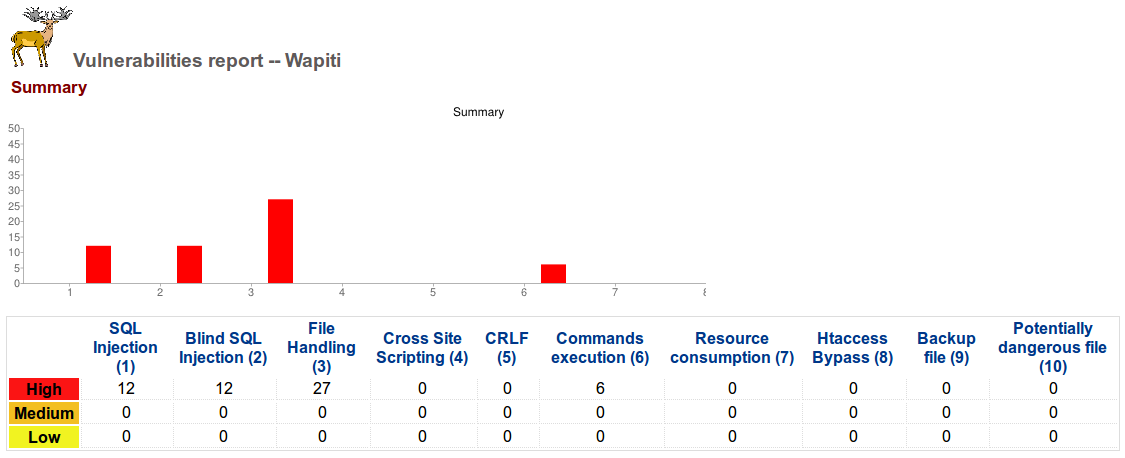
\includegraphics[width=\textwidth]{img/wapiti}
\caption{Il report generato dal tool Wapiti}
\end{figure}

Sono state individuate in tutto 57 vulnerabilità.
Ognuna delle vulnerabilità segnala che, ad una richiesta particolare, il server ha risposto con un codice d'errore \emph{500}\footnote{Questo codice d'errore indica un errore generico avvenuto sul server a seguito di una richiesta impossibile da risolvere(Internal server error).}.

\item \textbf{Exploit-me}\footnote{\url{http://labs.securitycompass.com/exploit-me/}}\\
Access-me non compatibile con Firefox 13
\item \textbf{Skipfish}\footnote{\url{http://code.google.com/p/skipfish/}}\\
Skipfish è un software ...

La versione testata è la 2.07b.

Per il corretto funzionamento dell'applicazione è stato necessario compilare i sorgenti con i seguenti comandi:

\small
{\tt  \# sudo apt-get install build-essential libssl-dev libdn11-dev\\
\# make\\
}

Una volta compilato Skipfish, è necessario configurare i dizionari.
Skipfish costruisce e mantiene automaticamente dei dizionari basati su URL e sui contenuti HTML incontrati nella scansione di un sito.
Questi dizionari sono particolarmente importanti per scansioni successive dello stesso sito.


\end{itemize}
\subsubsection{Tabelle e descrizione di rischi, probabilità e impatto}
Descrizione della nostra visione riguardante la probabilità dello sfruttamento di una vulnerabilità, l'impatto che questa vulnerabilità può avere sul sistema, e il grado di rischio che si corre.
\begin{center}
\begin{tabular}[t]{|p{1.5cm}|p{10cm}|}
\hline
\multicolumn{2}{|c|}{\bf Impatto} \\
\hline
Impatto & Descrizione \\
\hline
\hline
Alto & Significa che l'impatto dell'evento malevolo porterebbe ad una quasi totale compromissione del sistema, con conseguente perdita di riservatezza, integrità, e disponibilità dei dati. \\
\hline
Medio & Comporta che un evento malevolo potrebbe scatenare una perdita di dati media, cioè potrebbe portare alla perdita di riservatezza dei dati, o di disponibilità, senza intaccarne l'integrità.  \\
\hline
Basso   & Significa che un evento malevolo etichettato con questo livello di impatto non porterebbe problemi all'integrità delle informazioni del portale, portando a perdita di dati di non elevato interesse, oppure a una perdità di disponibilità temporanea. \\
\hline
\end{tabular}

%
\vspace{5mm}
%
\noindent %\hspace*{10pt}
\begin{tabular}[t]{|p{1.5cm}|p{10cm}|}
\hline
\multicolumn{2}{|c|}{\bf Probabilità} \\
\hline
Probabilità & Descrizione \\
\hline
\hline
Alta   & Significa che vi è un'alta probabilità che un agente malevolo possa facilmente avere l'opportunità di eseguire un attacco e che quest'ultimo vada a buon fine. \\
\hline
Mediia & Significa che vi è una media probabilità che l'agente abbia le capacità di eseguire determinati attacchi e di portarli a buon termine, e anche in caso vi riesca è molto probabile che le misure di sicurezza diano i propri frutti. \\
\hline
Bassa   & Significa che un agente ha poche probabilità di eseguire un attacco (per mancanza di conoscenze o capacità) e di portarlo a buon termine. Bassa probabilità sta anche a indicare che le misure di sicurezza prevengono totalmente un determinato tipo di attacco. \\
\hline
\end{tabular}
\end{center}

\vspace{5mm}

\begin{center}
\begin{tabular}{|l|c|c|c|}
\hline
\multicolumn{4}{|c|}{{\bf Livello di rischio}} \\
\hline
{{\bf Probabilità}} & \multicolumn{3}{c|}{{\bf Impatto}} \\ \cline{2-4}
     & Basso & Medio & Alto \\  \hline
 Alta & Basso & Medio & Alto  \\
\hline
 Medio & Basso & Medio & Medio \\
\hline
 Bassa & Basso & Basso & Basso \\
\hline
\end{tabular}
\end{center}

\subsubsection{{\it Valutazione del portale iMovies}}
Valutazione riguardante la parte software del portale iMovies, quindi tutte le possibilità di attacchi presi in considerazione e le contromisure per evitarli. Inoltre viene inserita una valutazione generale della probabilità, dell'impatto e del rischio dovuto a un determinato attacco. Per farlo ci si è affidati alla Top 10 dei rischi nelle web application del 2010 \cite{owasp} e al CAPEC.\\ 
\noindent
\begin{footnotesize}
\begin{longtable}{p{0.3cm}p{3cm}p{4.6cm}p{0.5cm}p{0.5cm}p{0.5cm}}
%\begin{tabular}
No. & Threat & Impl./planned countermeasure(s) & L & I & Risk \\
\hline
 1 & Cross Site Request Forgery & JSF 2.0 ha già incorporato un sistema di prevenzione al CSRF. Si tratta di {\tt javax.faces.ViewState}, un campo nascosto nel form. Usa valore autogenerato robusto come prevenzione al CSRF. & {\it Medio} & {\it Alto} & {\it Basso} \\
\hline
 2 & Cross-Site Scripting & JSF 2.0 ha già incorporato un sistema di prevenzione al XSS. JSF fa l'escape nella visualizzazione di un campo inserito dall'utente. {\tt <h:outputText/>} e {\tt <h:outputLabel/>} hanno un attributo {\tt escape="true"} di default e che quindi si può omettere. Si può anche scrivere {\tt<p>Welcome, \#{user.name}</p>} che viene automaticamente sanitizzato. & {\it Medio} & {\it Alto} & {\it Medio} \\
\hline
3 & Cross-Site Scripting & Protezione dei cookies. Per proteggere i cookies da Javascript maligni, i web server supportano la feature di permettere all'applicazione di specificare se un determinato cookie può essere acceduto da Javascript o solo da Http. Questa funzionalità è stata abilitata per tutte le app in {\tt conf/context.xml} aggiungendo {\tt <Context useHttpOnly="true">} & {\it Medio} & {\it Alto} & {\it Medio} \\
\hline
 4 & Sql Injection & Questo tipo di attacco non è responsabilità di JSF. Per ovviarlo usiamo query parametrizzate, utilizzando i {\tt PreparedStatement} di java per passare i parametri. & {\it Alta} & {\it Medio} & {\it Alto}\\
\hline
 5 & Broken Authentication and Session Management  & Per ovviare a questo tipo di attacco le sessioni sono dotate di un \emph{timeout} di 5 minuti che invalida e distrugge la sessione. Inoltre al logout dal sistema ogni sessione viene invalidata.
 & {\it Media} & {\it Medio} & {\it Alto}\\
\hline
 6 & Security Misconfiguration & Tutte le password standard di Apache Tomcat sono state modificate. Credenziali di default modificate. Errori gestiti in modo che alla richiesta di pagine non esistenti si venga re-indirizzati in una pagina di errore. Attivazione SSL su Apache Tomcat. & {\it Media} & {\it Medio} & {\it Alto}\\
\hline
 7 & Failure to Restrict URL Access & compila pure mattia :D & {\it Media} & {\it Medio} & {\it Alto}\\
\hline
 8 & Insufficient Transport Layer Protection & Grazie alle \emph{navigation rule} presenti nel file {\tt faces-config.xml} dell'applicazione, le regole di redirect sono ben definite da e per ogni pagina.  & {\it Media} & {\it Basso} & {\it Medio} \\
\hline
%%\end{tabular}
\end{longtable}
\end{footnotesize}



\subsubsection{{\it Valutazione della macchina server iMovies}}
Piccola valutazione dei problemi che potrebbe avere il software della macchina server.\\ \noindent
\begin{footnotesize}
\begin{longtable}{p{0.3cm}p{2.3cm}p{5.5cm}p{0.5cm}p{0.5cm}p{0.5cm}}
No. & Threat & Implemented/planned countermeasure(s) & L & I & Risk \\
\hline
1 & Perdita di dati & Viene eseguito un backup incrementale giornaliero e orario, e uno totale ogni venerdi alle ore 11 di tutte le chiavi private e certificati della CA. I backup vengono inseriti in una cartella all'interno di { \tt /var/ftp/admin} non accedibile. & {\it Bassa} & {\it Alto} & {\it Medio} \\
\hline
2 & Accesso macchina e dati a malintenzionati & problema da sistemare. dobbiamo mettere che solo tomcat e root possono toccare le cartelle. & {\it Media} & {\it Alto} & {\it Medio} \\
\hline
3 & Impossibilità di accesso alla macchina server & \'E stato installato un demone SSH che permette l'accesso da remoto alla macchina server, permettendo operazioni di manutenzione da remoto. & {\it Media} & {\it Alto} & {\it Medio} \\
\hline
4 & Impossibilità di accesso alla macchina server & \'E stato installato un server FTP per il download dei backups da remoto. La cartella dove è in esecuzione il server FTP (che è la cartella contenente i backups) è in {\tt chroot()}. Significa che l'utente remoto vedrà quella cartella come radice. & {\it Media} & {\it Alto} & {\it Medio} \\
\hline
5 & Compromissione Web Server & Apache Tomcat offre la possibilità di eseguire lo shutdown del Web Server da remoto, creando una classe Java che crea una connessione socket sulla porta prestabilita e inviando una determinata password nel buffer. & {\it Media} & {\it Alto} & {\it Medio} \\
\hline
3 & dobbiamo pensarci & insieme domani & {\it Media} & {\it Alto} & {\it Medio} \\
\hline
3 & dobbiamo pensarci & insieme domani & {\it Media} & {\it Alto} & {\it Medio} \\
\hline
\end{longtable}
\end{footnotesize}

\subsubsection{Descrizione dettagliata delle contromisure scelte}
La scelta di Java Server Faces non è stata del tutto casuale, o dettata dalla presenza del linguaggio di programmazione Java già conosciuto da tutti noi.

L'utilizzare un framework è stata una scelta dovuta anche al fatto di avere a disposizione uno strumento che già implementasse delle contromisure agli attacchi più diffusi. Questo ci ha permesso oltre che ovviare all'implementazione ``personale'' di contromisure (come nel caso del CSRF) ma anche di disporre di contromisure già implementate e relativamente sicure, perchè già testate da molti utenti, e create appunto dagli stessi sviluppatori e progettisti.

In particolare avremmo piacere di soffermarci sull'implementazione di JSF di una delle contromisure sul Cross Site Request Forgery. \\ \\ \\
---------------------------------------------------------------\\
Spiegazione di un paio di contromisure nel dettaglio.\\

\subsubsection{Risk Acceptance}

List all medium and high risks, according to the evaluation above. For each risk, propose additional countermeasures that could be implemented to further reduce the risks.

meo docet:
meo ha provato a fare attaco csrf. per farlo sei andato a guardare che tipo di richiesta la pagina edit.xhtml faceva per modificare i dati di un utente. dopo questa analisi ho preso brutalmente la richiesta e l'ho fatta a mano con webscarab e si è visto che veniva soddisfatta.
la richiesta aveva da qualche parte dei : non codificati in urlencoded. 
dopodiche ho provato a replicarla creando una pagina web ad hoc e mi ero arenato in un problema di difficoltà nell'invio del simbolo di : perche continuava a codificarli e io non li volevo codificati. 
giunto alla mezza conclusione che non si potesse fare in html ma solo tramite una richiesta javascrpt ho notato che c'era un campo che si chiama javax. state ecc che contenteva un numeraccio che variava ad ogni richiesta. sono andato a investigare quel campo e a ricercare se jsf implementasse gia sistemi contro csrfe ho scoperto che lo fa. 
\\ \\ 
-------------------------------------------
\\ \\ 

%\begin{footnotesize}
%\begin{prettytablex}{p{2cm}X}
%No. of threat & Proposed countermeasure including expected impact  \\
%\hline
%... & ... \\
%\hline
%... & ... \\
%\hline
%\end{prettytablex}
%\end{footnotesize}
\begin{thebibliography}{9}
\bibitem{applied security}
David Basin, Patrick Schaller, Micheal Schl\"apfer - Springer - \textit {Applied Information Security - A Hands-on Approach}
\bibitem{owasp}
OWASP - The ten most critical web application security risk 2010 - \href{http://owasptop10.googlecode.com/files/OWASP\%20Top\%2010\%20-\%202010.pdf}{OWASP Top Ten for 2010}
 
%Documento rilasciato dall'OWASP contenente la top ten dei rischi alla sicurezza più critici nelle Web Application nel 2010 
\end{thebibliography}
\end{document}

%%% Local Variables: 
%%% mode: latex
%%% TeX-master: "../../book"
%%% End: 
